\hypertarget{an-example-of-model-non-linearity-in-the-presence-of-a-linear-predictor.}{%
\section{An example of model non-linearity in the presence of a linear
predictor.}\label{an-example-of-model-non-linearity-in-the-presence-of-a-linear-predictor.}}
\label{sup:nomlinviol}

Notebook available on-line:

https://github.com/spisakt/mlconfound\_manuscript/tree/main/simulated/normality\_and\_linearity\_violation.ipynb

\begin{lstlisting}[language=Python]
import numpy as np
import seaborn as sns
import matplotlib.pyplot as plt
from sklearn.linear_model import Ridge
sns.set(rc={"figure.figsize":(6, 2)})
sns.set_style("white")
\end{lstlisting}

\hypertarget{five-features-one-linear-four-sigmoid}{%
\subsubsection{Five features: one linear, four
sigmoid}\label{five-features-one-linear-four-sigmoid}}

\begin{lstlisting}[language=Python]
n=300
p=5
rng = np.random.default_rng(42)
y = np.arange(n)
y = (y - y.mean())/y.std()

X_true = np.repeat(y, p).reshape(n,p)
for i in range(1,4):
    X_true[:,i] = np.tanh(X_true[:,i]*2)

X=X_true + rng.normal(0,0.1, (n,p))

for i in range(4):
    sns.lineplot(x=y, y=X_true[:,i])
    sns.scatterplot(x=y, y=X[:,i])
    plt.show()
\end{lstlisting}

\begin{figure}[H]
\centering
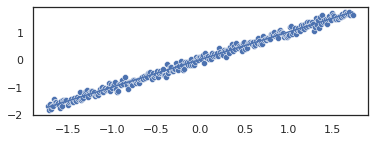
\includegraphics[width=0.15\paperwidth]{fig/normality_and_linearity_violation_files/normality_and_linearity_violation_3_0.png}
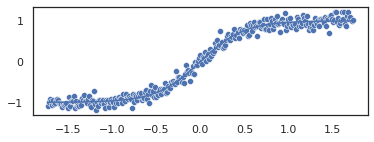
\includegraphics[width=0.15\paperwidth]{fig/normality_and_linearity_violation_files/normality_and_linearity_violation_3_1.png}
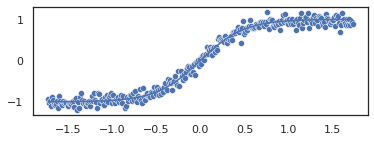
\includegraphics[width=0.15\paperwidth]{fig/normality_and_linearity_violation_files/normality_and_linearity_violation_3_2.png}
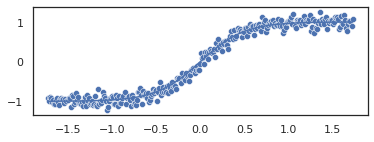
\includegraphics[width=0.15\paperwidth]{fig/normality_and_linearity_violation_files/normality_and_linearity_violation_3_3.png}
\end{figure}

\hypertarget{model-predictions-without-regularization}{%
\subsubsection{\texorpdfstring{Model predictions \textbf{without}
regularization}{Model predictions without regularization}}\label{model-predictions-without-regularization}}

\begin{lstlisting}[language=Python]
model = Ridge(alpha=0)
model.fit(y=y, X=X)
yhat = model.predict(X)
sns.scatterplot(x=y, y=yhat, alpha=0.3)
model.coef_
\end{lstlisting}

\begin{lstlisting}
array([ 0.47902429,  0.00946499,  0.07378478, -0.02828672,  0.47070535])
\end{lstlisting}

\begin{figure}[H]
\centering
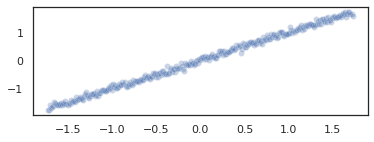
\includegraphics[width=0.5\paperwidth]{fig/normality_and_linearity_violation_files/normality_and_linearity_violation_5_1.png}
\end{figure}

\hypertarget{model-predictions-with-regularization}{%
\subsubsection{\texorpdfstring{Model predictions \textbf{with}
regularization}{Model predictions with regularization}}\label{model-predictions-with-regularization}}

\begin{lstlisting}[language=Python]
model = Ridge(alpha=2000)
model.fit(y=y, X=X)
yhat = model.predict(X)
sns.scatterplot(x=y, y=yhat, alpha=0.3)
model.coef_

\end{lstlisting}

\begin{lstlisting}
array([0.09472368, 0.07472972, 0.07338482, 0.07440682, 0.09463765])
\end{lstlisting}

\begin{figure}[H]
\centering
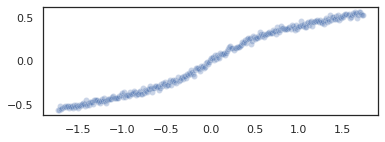
\includegraphics[width=0.5\paperwidth]{fig/normality_and_linearity_violation_files/normality_and_linearity_violation_7_1.png}
\end{figure}
